\documentclass[fontset=none]{Notes}

\makeatletter
\DeclareRobustCommand{\em}{%
  \@nomath\em \if b\expandafter\@car\f@series\@nil
  \normalfont \else \bfseries \fi}
\makeatother

\usepackage{tikz-cd,tkz-graph}
\usepackage{siunitx,tikz,nicematrix}
\usetikzlibrary{matrix,calc}

\ProvidesFile{font.def}

\setCJKmainfont{Source Han Serif SC}[
  UprightFont=*-Regular,
  BoldFont=*-Bold,
  ItalicFont=HYKaiTi S,
  ItalicFeatures={Scale=1.1}
]
\newCJKfontfamily[zhsong]\songti{Source Han Serif SC}[
  UprightFont=*-Regular,
  BoldFont=*-Bold,
  ItalicFont=HYKaiTi S,
  ItalicFeatures={Scale=1.1}
]
\setCJKsansfont{Source Han Sans SC}[
  UprightFont=*-Regular,
  BoldFont=*-Bold
]
\newCJKfontfamily[zhhei]\heiti{Source Han Sans SC}[
  UprightFont=*-Regular,
  BoldFont=*-Bold
]
\setCJKmonofont{HYFangSong S}[
  BoldFont=*,
  ItalicFont=*,
  BoldItalicFont=*
]
\newCJKfontfamily[zhfs]\fangsong{HYFangSong S}[
  BoldFont=*,
  ItalicFont=*,
  BoldItalicFont=*
]
\newCJKfontfamily[zhkai]\kaishu{HYKaiTi S}[
  BoldFont=*,
  ItalicFont=*,
  BoldItalicFont=*
]

\setmainfont{texgyretermes}[
  Extension=.otf,
  UprightFont=*-regular,
  BoldFont=*-bold,
  ItalicFont=*-italic,
  BoldItalicFont=*-bolditalic,
  SlantedFont=*-italic
]
%\setmathrm{texgyretermes}[
%  Extension=.otf,
%  UprightFont=*-regular,
%  BoldFont=*-bold,
%  ItalicFont=*-italic,
%  BoldItalicFont=*-bolditalic,
%  SlantedFont=*-italic
%]
\setsansfont{Cantarell}[
  UprightFont=* Regular,
  ItalicFont=* Italic,
  BoldFont=* Bold,
  BoldItalicFont=* Bold Italic,
  SmallCapsFont=Alegreya Sans SC
]
\setmonofont{Ubuntu Mono}[
  UprightFont=*,
  ItalicFont=* Italic,
  BoldFont=* Bold,
  BoldItalicFont=* Bold Italic
]
%\setmathfont{texgyretermes-math.otf}
%\setmathfont[range={\mathcal,\mathbfcal,\mathfrak},StylisticSet=1]{XITSMath-Regular.otf}
%\setmathfont[range={\mathbb}]{KpMath-Sans.otf}



\usepackage[subscriptcorrection,nofontinfo,mtpbb,mtpfrak]{mtpro2}
\usepackage[normal]{fixdif}

\tikzcdset{
  arrow style=tikz,
  diagrams={>={Straight Barb[scale=0.8]}}
}

\tikzset{
  >={latex}
}

\allowdisplaybreaks[1]

\newlength{\mymathln}
\newcommand{\aligninside}[2]{
  \settowidth{\mymathln}{#2}
  \mathmakebox[\mymathln]{#1}
}

\DeclareMathOperator\Ad{Ad}
\DeclareMathOperator\ad{ad}
\DeclareMathOperator\im{im}
\DeclareMathOperator\sgn{sgn}
\DeclareMathOperator\rad{rad}
\DeclareMathOperator\Alt{Alt}
\DeclareMathOperator\Max{Max}
\DeclareMathOperator\GL{GL}
\DeclareMathOperator\SL{SL}
\DeclareMathOperator\Orth{O}
\DeclareMathOperator\U{U}
\DeclareMathOperator\SpO{SO}
\DeclareMathOperator\SU{SU}
\DeclareMathOperator\Lie{Lie}
\DeclareMathOperator\End{End}
\DeclareMathOperator\Int{Int}
\DeclareMathOperator\Sym{Sym}
\DeclareMathOperator\tr{tr}
\DeclareMathOperator\Hom{Hom}
\DeclareMathOperator\supp{supp}
\DeclareMathOperator\Id{Id}
\DeclareMathOperator\rk{rank}
\DeclareMathOperator\grad{grad}
\DeclareMathOperator\Euc{E}
\DeclareMathOperator\SE{SE}
\DeclareMathOperator\spn{span}
\DeclareMathOperator\dive{div}
\DeclareMathOperator\curl{curl}
\DeclareMathOperator*\argmax{argmax}
\newcommand{\LL}{{\mathrm{L}}}

\newcommand{\ideal}[1]{\mathfrak{#1}}
\newcommand{\norm}[1]{\left\lVert#1\right\rVert}
\newcommand{\mat}[1]{\mathbold{#1}}
\newcommand{\uline}{\underline{\hphantom{X}}}
\newcommand{\abs}[1]{\left|#1\right|}
\newcommand{\lie}[1]{\mathfrak{#1}}
\newcommand{\inn}[1]{\left\langle #1\right\rangle}

\usepackage{enumitem}

\setlist[enumerate]{nosep}

%\DeclareMathAlphabet\mathcal{OMS}{cmsy}{m}{n}
\DeclareMathSymbol{\into}{\mathbin}{AMSa}{"79}

\newlength\stextwidth
\newcommand\makesamewidth[3][c]{%
  \settowidth{\stextwidth}{#2}%
  \makebox[\stextwidth][#1]{#3}%
}

\usepackage{minted}

\begin{document}

\frontmatter

\tableofcontents

\mainmatter

\chapter{导论}

\section{机器人学中的推理问题}

要在现实世界中明智行事,机器人需要从传感器数据中推断出关于世界的知识,同时借助先验知识。机器人学中存在诸多此类推断问题,但没有任何一个能像同步定位与建图(SLAM)这样获得如此广泛的关注。我们将详细探讨SLAM技术,并以其作为后续论述的典型案例。其他推断问题包括已知环境中的定位、对环境其他活动体的追踪,以及上述所有问题的多机器人协同版本。更专业化的课题同样值得关注,例如标定技术或长期惯性导航。

在SLAM问题中,核心目标是通过机器人传感器获取的信息实现机器人定位。简单场景下,这可能表现为对一组路标点的方位测量。若路标位置已知,这就转化为类似于船舶海上导航的三角测量问题。然而SLAM的独特挑战在于:我们并不预先掌握路标地图,因此必须在动态构建地图的过程中,同步完成对未知地图的推断与基于该演进地图的定位。

图~\ref{fig:toy slam} 展示了一个简单的示例,说明了该问题的结构。位于连续三个位姿 $x_1,x_2,x_3$ 
的机器人对两个地标 $l_1,l_2$ 进行了方位观测。为了将解固定在空间中,
我们假设第一个位姿 $x_1$ 存在绝对位置/方向测量。若缺少该测量,
由于所有方位观测都是相对的,将无法获取绝对位置信息。

\begin{figure}[htb]
  \centering
  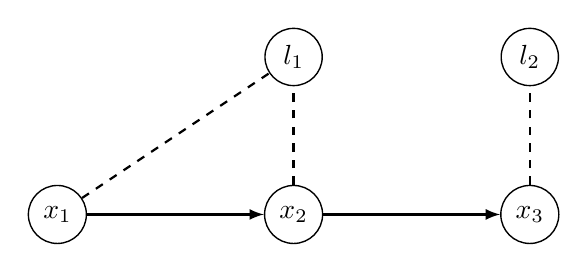
\begin{tikzpicture}
    \GraphInit[vstyle=Normal]
    \SetGraphUnit{3}
    \SetVertexMath
    \Vertices{line}{x_1,x_2,x_3}
    \SetGraphUnit{2}
    \NO(x_2){l_1}
    \NO(x_3){l_2}
    \Edges[style=->](x_1,x_2,x_3)
    \Edge[style=dashed](x_1)(l_1)
    \Edge[style=dashed](x_2)(l_1)
    \Edge[style=dashed](x_3)(l_2)
  \end{tikzpicture}
  \caption{一个玩具级SLAM(同步定位与建图)示例,
  包含三个机器人位姿和两个地标点。我们用箭头示意机器人运动轨迹,
  虚线则表示方位测量关系。}\label{fig:toy slam}
\end{figure}

\section{概率建模}

由于测量存在不确定性,我们无法期望还原世界的真实状态,但可以通过概率
描述来推断测量结果所蕴含的信息。在贝叶斯概率框架下,我们运用概率论的语言
对不确定事件赋予主观置信度。本节末尾列有多部优秀著作深入探讨这一主题,鉴于
篇幅所限,此处不再赘述。

在机器人学中,我们通常需要对连续的多维随机变量 $x\in \mathbb{R}^n$
建立置信度模型。我们使用概率密度函数 $p(x)$ 来表述,其满足
\[
  \int p(x)\d x=1.
\]

在 SLAM 中,我们希望在给定一组观测测量值 $Z$ 的情况下,描述关于未知量 $X$
(此处指机器人位姿与未知地标位置)的认知状态。用贝叶斯概率的术语来说,
这就是简单的条件概率密度
\[
  p(X|Z).
\]
这样的描述被称为概率推断。前提是首先为感兴趣的变量指定一个概率模型,
并说明它们如何产生(不确定的)测量结果。这正是概率图模型发挥作用的地方。

\emph{概率图模型}通过利用数据的结构,提供了一种简洁描述复杂概率密度的机制。
具体而言,高维概率密度通常可分解为多个因子的乘积,每个因子都是定义在更小域
上的概率密度。当我们稍后在本节引入因子图时,将对此进行明确建模。

\section{生成式建模的贝叶斯网络}

贝叶斯网络是一种用于建模机器人学中推理问题的便捷图形语言。
这是因为我们通常很容易理解传感器如何生成测量数据。举例来说,若已知地标
的精确位置、机器人位姿及其传感器配置的几何结构,便不难预测应获得何种测量结果。
我们既可以假设也能通过学习获得特定传感器的噪声模型。测量预测与噪声模型构成了
生成式模型的核心要素,这与贝叶斯网络框架高度契合。

通常而言,\emph{贝叶斯网络}(或称贝叶斯网)是一种有向图模型,其节点代表变量 $\theta_j$。
我们记感兴趣的随机变量集合为 $\Theta=\{\theta_1,\dots,\theta_n\}$。
一个贝叶斯网络定义了在所有变量上的联合概率密度 $p(\Theta)$,其定义为
相对于每个节点的条件概率密度的乘积:
\[
  p(\Theta)=\prod_{j} p(\theta_j|\pi_j).
\]
上述公式中 $\pi_j$ 是赋予 $\theta_j$ 的父节点的一个值。
因此,在贝叶斯网络中,联合概率密度的分解方式由其图结构决定,特别是节点-父节点的关系所主导。

例如,让我们考虑与图~\ref{fig:toy slam} 中玩具 SLAM 示例相关的贝叶斯网络。
在这种情况下感兴趣的随机变量集合为 $\Theta=\{X,Z\}$,$X$ 表示未知的位姿和
路标点,$Z$ 表示测量值。这个玩具示例对应的贝叶斯网络如图~\ref{fig:bayes net of toy slam} 所示,其中
方形盒子表示观测值。根据贝叶斯网络的一般定义,联合概率密度
$p(X,Z)=p(x_1,x_2,x_3,l_1,l_2,z_1,z_2,z_3,z_4)$ 是通过下述条件概率密度的乘积得到的:
\begin{align}
  p(X,Z)&=p(x_1)p(x_2|x_1)p(x_3|x_2)\label{eq:markov of pose}\\
  &\times p(l_1)p(l_2) \label{eq:density of landmarks}\\
  &\times p(z_1|x_1) \label{eq:meas on x1}\\
  &\times p(z_2|x_1,l_1)p(z_3|x_2,l_1)p(z_4|x_3,l_2). \label{eq:meas on x}
\end{align}
可以看出,这种情况下的联合密度由四组性质迥异的因子构成:
\begin{itemize}
  \item 位姿 $x_1,x_2,x_3$ 上的“Markov 链” $p(x_1)p(x_2|x_1)p(x_3|x_2)$,即 
  \eqref{eq:markov of pose} 式。条件概率密度 $p(x_{t+1}|x_t)$ 可能表示
  先验知识或者由已知的控制输入得到的信息。
  \item 路标点 $l_1,l_2$ 的先验概率密度 $p(l_1),p(l_2)$,即 \eqref{eq:density of landmarks} 式。
  (当没有先验地图的时候通常在 SLAM 设置中忽略)
  \item 对应于第一个位姿 $x_1$ 上的绝对位姿测量的条件概率密度 $p(z|x_1)$,
  即 \eqref{eq:meas on x1} 式。
  \item 对应于位姿 $x_1,x_2,x_3$ 对路标点 $l_1,l_2$ 的三个方位测量的条件
  概率密度的乘积 $p(z_2|x_1,l_1)p(z_3|x_2,l_1)p(z_4|x_3,l_2)$,
  即 \eqref{eq:meas on x} 式。
\end{itemize}

需要注意的是,图结构对数据关联做出了明确声明,即对于每个测量值 $z_k$,
我们都清楚它是对哪个地标的测量。虽然在图模型框架下可以对未知数据关联进行建模,
但在本文中,我们假设数据关联是通过预处理步骤获得的结果。

\begin{figure}[htb]
  \centering
  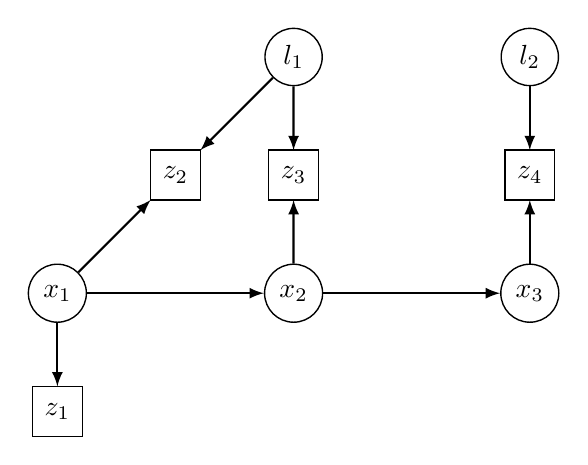
\begin{tikzpicture}
    \GraphInit[vstyle=Normal]
    \SetGraphUnit{3}
    \SetVertexMath
    \Vertices{line}{x_1,x_2,x_3}
    \NO(x_2){l_1}
    \NO(x_3){l_2}
    \SetVertexNormal[Shape=rectangle]
    \coordinate (z_2) at ($(x_1)!.5!(l_1)$) {};
    \coordinate (z_3) at ($(x_2)!.5!(l_1)$) {};
    \coordinate (z_4) at ($(x_3)!.5!(l_2)$) {};
    \Vertex[Node]{z_2}
    \Vertex[Node]{z_3}
    \Vertex[Node]{z_4}
    \SetGraphUnit{1.5}
    \SO(x_1){z_1}
    \Edges[style=->](x_1,x_2,x_3)
    \Edge[style=->](x_1)(z_2)
    \Edge[style=->](l_1)(z_2)
    \Edge[style=->](x_2)(z_3)
    \Edge[style=->](l_1)(z_3)
    \Edge[style=->](x_3)(z_4)
    \Edge[style=->](l_2)(z_4)
    \Edge[style=->](x_1)(z_1)
  \end{tikzpicture}
  \caption{对应图~\ref{fig:toy slam} 中的贝叶斯网络示例。
  我们用方形节点表示测量值,因为这些变量通常是可观测的。}\label{fig:bayes net of toy slam}
\end{figure}

\section{特定的概率密度}

上述密度函数的具体形式在很大程度上取决于应用场景和所使用的传感器。
最常用的密度函数是多元高斯分布,其概率密度为
\[
  \mathcal{N}(\theta;\mu,\Sigma)=\frac{1}{\sqrt{|2\pi\Sigma|}}
  \exp\left(-\frac{1}{2}\norm{\theta-\mu}_{\Sigma}^2\right),
\]
其中 $\mu\in \mathbb{R}^n$ 是均值,$\Sigma$ 是 $n\times n$ 协方差矩阵,
以及
\[
  \norm{\theta-\mu}_{\Sigma}^2=(\theta-\mu)^\top\Sigma^{-1}(\theta-\mu)
\]
是 Mahalanobis 距离的平方。例如,未知量的先验通常使用高斯密度函数来指定。

在许多情况下,将测量值建模为零均值高斯噪声既是合理的也是方便的。例如,
从给定位姿 $x$ 到特定地标 $l$ 的方位测量值就可以这样建模为
\[
  z=h(x,l)+\eta,
\]
其中 $h$ 是量测函数,噪声 $\eta$ 来源于具有协方差 $R$ 的零均值高斯密度分布。
这导出了量测 $z$ 上的条件概率密度 $p(z|x,l)$ 为
\[
  p(z|x,l)=\mathcal N(z;h(x,l),R)=\frac{1}{\sqrt{|2\pi R|}}\exp\left(
    -\frac{1}{2}\norm{h(x,l)-z}_R^2
  \right).
\]

在实际机器人应用中,测量函数 $h$ 通常是非线性的。尽管这些函数取决于实际使用的传感器,但通常不难推导或书写。
二维方位测量的测量函数可简单表示为
\[
  h(x,l)=\arctan(l_y-x_y,l_x-x_x),
\]
其中 $\arctan$ 表示计算机中的 \mintinline{text}{atan2} 函数。因此,最终的概率测量模型
$p(z|x,l)$ 可以表示为
\begin{equation}\label{eq:pzxl}
  p(z|x,l)=\frac{1}{\sqrt{|2\pi R|}}\exp\left(
    -\frac{1}{2}\norm{\arctan(l_y-x_y,l_x-x_x)-z}_R^2
  \right).
\end{equation}
需要注意的是,我们并不总是假设测量噪声服从高斯分布:例如为了应对偶发性的数据关联错误,
许多学者提出了采用鲁棒性测量密度函数的方法,这类函数比高斯密度具有更厚的尾部特征。

并非所有涉及的概率密度都源自测量数据。例如,在玩具 SLAM 问题中,我们拥有形如 $p(x_{t+1}|x_t)$ 的
概率密度函数,它规定了机器人被假定遵循的概率运动模型。这可以通过里程计测量得出,在这种情况下
我们将完全按照上述描述进行操作。或者,这种运动模型可能源自已知的控制输入 $u_t$。在实际应用中,
我们通常采用条件高斯假设,
\[
  p(x_{t+1}|x_t,u_t)=\frac{1}{\sqrt{2\pi Q}}\exp\left(
    -\frac{1}{2}\norm{g(x_t,u_t)-x_{t+1}}_Q^2
  \right),
\]
其中 $g$ 是运动模型,$Q$ 是一个适当维度的协方差矩阵,例如在平面操作的机器人情况下为 $3×3$。需要注意的是,
对于在三维空间操作的机器人,我们将需要稍微更复杂的机制来指定非线性流形(如 $\SE(3)$)上的密度,如第 6 节所述。

\section{依据贝叶斯网络的仿真}

值得一提的是,一旦概率模型被指定为贝叶斯网络,从中进行模拟就变得轻而易举。这正是贝叶斯网络成为生成建模首选语言的原因。
我们在此提及这一点,因为在构建模型时考虑这个特性往往大有裨益。

具体而言,要从 $P(\Theta) =\prod_j  P(\theta_j |\pi_j )$ 中进行仿真,只需对图中的节点进行拓扑排序,
并以这样的方式进行采样:在从条件分布 $P(\theta_j |\pi_j )$ 中采样 $\theta_j$ 之前,先生成所有
父节点的值 $\pi_j$,这一过程总是可行的。该技术被称为祖先采样。

例如,让我们再次考虑玩具 SLAM 问题。即使在这个微小的问题中,也能明显看出联合密度的因式分解如何让我们进行局部的思考,
而不必考虑全局。事实上,我们可以利用图~\ref{fig:bayes net of toy slam} 中的贝叶斯网络作为指导,
对于联合密度 $p(x_1, x_2, x_3, l_1, l_2, z_1, z_2, z_3, z_4)$,我们分别进行:
\begin{enumerate}
  \item 从 $p(x_1)p(x_2|x_1)p(x_3|x_2)$ 中采样位姿 $x_1,x_2,x_3$(仿真机器人轨迹);
  \item 从 $p(l_1),p(l_2)$ 中采样路标点 $l_1,l_2$ (生成合理的路标点);
  \item 从条件密度 $p(z_1|x_1),p(z_2|x_1,l_1),p(z_3|x_2,l_1),p(z_4|x_3,l_2)$ 中采样测量值
  (仿真机器人的传感器)。
\end{enumerate}
许多其他拓扑排序方式也是可行的。例如,上述步骤 1 和 2 可以互换顺序而不影响结果。
此外,我们可以在生成 $x_1$ 之后的任意时刻生成位姿测量值 $z_1$,等等。

\section{最大后验推断}

既然我们已经掌握了为世界建模的方法,就能在获得相关信息时推断出关于世界的知识。前文我们已了解如何
通过贝叶斯网络完整定义联合概率密度 $P(\Theta)$:其因式分解由网络图结构决定,而精确计算形式则通过指定先验
分布与条件概率密度来实现。

在机器人学领域,我们通常关注的是在给定观测数据 $Z$ 的情况下,未知状态变量 $X$(如位姿和路标)的估计问题。
针对这些未知状态变量 $X$,最常用的估计器是最大后验概率估计(MAP),其命名源于该方法通过最大化给定观测数据
$Z$ 时状态变量 $X$ 的后验概率密度 $p(X|Z)$ 来实现估计:
\[
  X^{\mathrm{MAP}}=\argmax_X p(X|Z)=\argmax_X\frac{p(Z|X)p(X)}{p(Z)}.
\]

然而,贝叶斯定律的另一种表达形式才是理解 MAP 推断背后真实计算过程的关键。事实上,上式中所述
贝叶斯定律的所有量理论上都可以通过贝叶斯网络计算得出。但由于测量值 $Z$ 是给定的,归一化因子
所以 $p(Z)$ 对最大化过程无关紧要,可以忽略。此外,虽然条件概率密度 $p(Z|X)$ 关于 $Z$ 是经过适当归一化的高斯密度,
但我们只关注它作为未知状态 $X$ 的函数形式。因此,贝叶斯定律的第二种且更为重要的形式是:
\[
  X^{\mathrm{MAP}}=\argmax_X l(X;Z) p(X).
\]
这里 $l(X;Z)$ 是给定量测 $Z$ 下的状态 $X$ 的极大似然,其定义为与 $p(X|Z)$ 
成比例的任意函数:
\[
  l(X;Z)\varpropto  p(Z|X).
\]
记号 $l(X;Z)$ 是为了强调这个极大似然是 $X$ 的函数而不是 $Z$ 的函数。

需要认识到的是,基于测量结果的条件化处理所产生的似然函数通常并不呈现高斯分布形态。
为说明这一点,让我们重新审视公式 \eqref{eq:pzxl} 中的二维方位测量的密度函数。
当将其改写为似然函数时,我们得到
\[
  l(X;Z)\varpropto \exp\left(
    -\frac{1}{2}\norm{\arctan(l_y-x_y,l_x-x_x)-z}_R^2
  \right),
\]
这是关于 $z$ 的高斯分布,但是不是关于 $x$ 的。即使对于线性测量函数,测量值 $z$ 的维度
通常也低于其所依赖的未知变量的维度。因此,以其为条件最多只能在未知数上产生退化的
高斯密度;只有当我们融合多个测量信息时,未知数上的密度才会成为一个合理的概率密度。
在测量数据不足以完全约束所有变量的情况下,MAP 推断将失效,因为无法获得
后验概率的唯一最大化解。

上述所有内容促使我们在下一节引入因子图。引入新图形建模语言的原因在于:(a) 状态
$X$ 与测量值 $Z$ 之间存在明显区分;(b) 我们更关注非高斯似然函数这一
事实---这些函数并非严格意义上的概率密度函数。因此,贝叶斯网络语言与我们实际
关注的优化问题匹配度较低。最后我们将在第 3 节看到,因子图的结构与解决大规模推理
问题的计算策略密切相关。

\section{用于推断的因子图}

虽然贝叶斯网络是优秀的建模语言,但因子图更适合执行推理任务。与贝叶斯网络类似,
因子图允许我们将联合密度表示为若干因子的乘积。然而其更具普适性---不仅能用于定义
变量集 $X$ 上的概率密度函数,还可表示任意因子分解形式的函数 $\varphi(X)$。

为了说明这一点,让我们考虑在玩具 SLAM 示例中进行最大后验概率推断。在给定观测值 
$Z$ 的条件下,后验概率 $p(X|Z)$ 可以表述为
\begin{align}
  p(X|Z)&\varpropto p(x_1)p(x_2|x_1)p(x_3|x_2)\label{eq:markov of pose 1}\\
  &\times p(l_1)p(l_2) \label{eq:density of landmarks 1}\\
  &\times l(x_1;z_1) \label{eq:meas on x1 1}\\
  &\times l(x_1,l_1;z_2)l(x_2,l_1;z_3)l(x_3,l_2;z_4). \label{eq:meas on x 1}
\end{align}










\end{document}
